\section{Investigation}
\label{sec:investigation}
We now use POSE to investigate the CPU power consumption of codes from the Mantevo~\cite{heroux:2009aa} and Rodinia~\cite{che:2009aa} benchmark suites.
The applications studied are simplified versions of production codes intended for research purposes.
As such they have relatively compact code bases and well understood behaviours while still providing representative workloads.

CPU energy consumption accounts for a significant portion of the energy used by high performance systems~\cite{rong:2010aa} and is therefore a prime target for optimisation.
It can also be measured accurately on commodity hardware~\cite{hackenberg:2013aa} making it a suitable candidate for POSE modelling.
Our experiments were carried out on an Intel Core i5-3470 Ivy Bridge CPU which supports Intel's Running Average Power Limit (RAPL) technology~\cite{david:2010aa}.

\subsection{CPU Power Consumption}
\label{ssec:cpupower}
Current processors are based on Complimentary Metal Oxide Semiconductor (CMOS) technology.
\autoref{eq:totpwr} separates the power draw of CMOS chips into its component parts, of which dynamic and leakage power are the most significant.
\begin{equation}
\label{eq:totpwr}
P_{tot} = P_{dyn} + P_{leak} + P_{other}
\end{equation}
Dynamic power is consumed when logic gates change state.
Leakage power exists because at microscopic scales the insulating properties of silicon break down, allowing some current to escape even when gates remain inactive.
Other forms of power dissipation exist, however their effects are relatively minor \cite{kaxiras:2008aa}.
\begin{gather}
P_{dyn} \propto CV^{2}Af \label{eq:dynpwr} \\
P_{leak} = V\times I_{leak} \label{eq:staticpwr}
\end{gather}
\autoref{eq:dynpwr} is a common approximation for dynamic power in which $C$ denotes load capacitance, $V$ the supply voltage, $A$ the activity factor and $f$ the clock frequency.
\autoref{eq:staticpwr} is a simplified expression for leakage power which exploits the fact that leakage current ($I_{leak}$) is invariant to processor workload~\cite{kim:2003aa}.

Activity factor captures the fraction of logic elements which change state each clock cycle.
Frequency and supply voltage vary in tandem, taking values from a set of $(frequency, voltage)$ pairs known as P-states.
Dynamic Voltage and Frequency Scaling (DVFS) selects a P-state based on workload, or places the CPU into an energy saving mode if no work is available.
Finally, capacitance and leakage current are constants dictated by hardware design.

Processor architecture also plays a significant roll in determining total power consumption.
Each core in a multi-core architecture operates independently with its own activity factor and in some cases P-state.
As a result, \autoref{eq:totpwr} should be summed across all cores to arrive at a value for the entire processor.

\subsection{Feasible Performance Envelope}
The first step in applying POSE is to construct a feasible performance envelope.
Many manufacturers publish power dissipation figures for their hardware, however for safety reasons these are usually conservative estimates.
POSE works best when the maximum and minimum power bounds are as tight as possible, therefore we determine $P_{\max}$ and $P_{\min}$ empirically.

We specify power benchmarks using $(S,A,C)$ tuples, with P-state $S$, activity factor $A$ and active core count $C$.
Our $P_{min}$ and $P_{max}$ benchmarks should reflect the range of values these properties can take for a given code $\theta$.
This notion is formalised by \autoref{eq:pbench}.
\begin{align}
  \label{eq:pbench}
  \begin{split}
    P_{min} &= (S_{min}, A_{min}, C_{min}~\vert~\theta), \\
    P_{max} &= (S_{max}, A_{max}, C_{max}~\vert~\theta) 
  \end{split}
\end{align}
The values of $S$, $A$, and $C$ depend on the code and the nature of the optimisations being considered.
POSE models for inherently serial codes should be constructed using single threaded benchmarks where $C_{min} = C_{max} = 1$, for example.

The \texttt{cpufrequtils} package allows us to override DVFS and manually set the desired P-state $S$.
We control the number of active cores $C$ by specifying the number of threads used by our benchmarking routines and pinning each one to its own core to prevent migration.
The remaining property is activity factor, which is influenced by benchmark code.

\begin{figure}[ht]
\centering
\lstset{basicstyle=\ttfamily\footnotesize\bfseries, frame=tb} %small bold text, lines top and bottom
\lstinputlisting[]{lst/alpha_benchmark.c}
\caption{Activity Factor $\alpha$ Benchmark Code}
\label{fig:microbench}
\end{figure}

We define the range of values that $A$ can take for some fixed $S$ and $C$ as $[\alpha,~\beta]$ where $0 < \alpha < \beta < 1$.
Our code for targeting activity factor $\alpha$ is given in \autoref{fig:microbench}.
This benchmark executes a single \texttt{jmp} instruction each clock cycle, preventing instruction pipelining.
It performs no floating point or integer calculations and no memory accesses whilst keeping control logic to a minimum.

Non-trivial codes perform more work per unit time than our minimal benchmark.
This additional work means more transistors changing state per cycle, and hence a higher activity factor.
The only exception occurs when applications are blocked for long periods, allowing the processor to enter an idle state.
This can be addressed by adding delays to the benchmark if necessary.

FIRESTARTER~\cite{hackenberg:2013ab} serves as our benchmark for activity factor $\beta$.
This tool is designed to trigger near-peak power consumption across a range of x86\_64 processors.
It consists of hand optimised assembly routines which raise activity factor above the level achievable with high level languages.
Prime95 and Linpack were also evaluated as potential $\beta$ benchmarks however they were consistently outperformed by FIRESTARTER.

The benchmark parameter space is small enough to fully characterise a processor by measuring all $(S,A,C)$ configurations.
Benchmarking runs lasted for 120 seconds to allow enough time for power readings to stabilise.
We extended the Unix \texttt{time} binary to gather power consumption figures using RAPL.
Techniques described by Hahnel~et~al.~\cite{hahnel:2012aa} were used to promote measurement accuracy.
Results are presented in \autoref{tab:fpe_params}, which identifies P-states by their frequency component.

\begin{table}
\centering
\caption{Feasible Performance Envelope Parameters (W)}
\label{tab:fpe_params}
\input{tab/tex/fpe_params.tex}
\end{table}

\subsection{POSE Models for Code Optimisation}
Having characterised our system we now proceed to build POSE models for applications in the Mantevo and Rodinia suites.
These codes were compiled with ICC version 14.0.0.
Codes were run with default configurations where available.
The energy and runtime costs associated with each code is given in \autoref{tab:code_metrics}.

\begin{table}
\centering
\caption{Code Metrics for $S = 3.2\text{ GHz}$, $C = 4$}
\label{tab:code_metrics}
\input{tab/tex/code_metrics.tex}
\end{table}

All codes ran in parallel across four cores.
They also spent a negligible amount of time waiting for resources. 
This allowed the CPU to run at its maximum supported frequency of 3.2 GHz.
For the first stage of this investigation we disregard optimisations which reduce parallelism ($C < 4$) or processor throughput (S < 3.2 GHz).
The benchmark configurations used were $(\text{3.2 GHz}, \alpha, 4)$ for $P_{min}$ and $(\text{3.2 GHz}, \beta, 4)$ for $P_{max}$, yielding power draws of 26.88W and 49.61W respectively.

\begin{table}
  \setlength{\tabcolsep}{.5em}
  \caption{$E^1t^2$ POSE Points}
  \begin{subtable}{\textwidth}
  \centering
  \caption{Time (s)}
  \input{tab/tex/code_pose_time.tex}
  \end{subtable}
  \begin{subtable}{\textwidth}
  \centering
  \caption{Energy (J)}
  \input{tab/tex/code_pose_energy.tex}
  \end{subtable}
  \label{tab:pose_params}
\end{table}

\autoref{tab:pose_params} summarises the POSE models constructed for each code.
The remainder of this section focusses on MiniMD and LavaMD as the two codes representing the extremes of power consumption.
POSE models for these two codes are reproduced graphically in \autoref{fig:minimd_pose} and \autoref{fig:lavamd_pose}.
When comparing these diagrams it is readily apparent that LavaMD offers far more scope for power optimisation than MiniMD, which offers virtually none. 
POSE provides the following insights for LavaMD:
\begin{itemize}
  \item At most 353.36J can be saved by reducing power consumption.
  \item The maximum slowdown from energy optimisation is 4.12s.
  \item The most power optimised value of $E^1t^2$ is 6332609, a 30.59\% reduction.
  \item A speed up of 8.77s, or $1.15 \times$, strictly outperforms $\theta$.
  \item A speed up of 15.29s, or $1.30 \times$, strictly outperforms any power optimisation.
\end{itemize}

\begin{figure}[t]%
  \providecommand{\plotwidth}{.95\linewidth}
  \begin{subfigure}[t]{.5\linewidth}%
    \begin{tikzpicture}
  \begin{axis}[
    axis on top,
    axis x line=bottom,
    axis y line=left,
    xlabel={Runtime (\emph{s})},
    ylabel={Energy (\emph{J})},    
    xmin=24, xmax=31,
    ymin=650, ymax=1650,
    width=0.80\linewidth,
    legend columns=3,
    legend to name=minimd:legend,
    legend style={/tikz/every even column/.append style={column sep=0.2cm}} % space out columns a bit
    ]

    %% Model Parameters %%
    \pgfmathsetmacro{\baselinepower}{26.876067}
    \pgfmathsetmacro{\rooflinepower}{49.60612}
    \pgfmathsetmacro{\codepower}{27.95947000000066} 
    \pgfmathsetmacro{\codetime}{30.293834}
    \pgfmathsetmacro{\codeenergy}{846.999542908}
    \pgfmathsetmacro{\energyexp}{1.0}
    \pgfmathsetmacro{\timeexp}{2.0}

    % Sadly, pgfplots sucks too much to calculate cube roots
    % These values are calculated with a ruby script in tools
    \pgfmathsetmacro{\blnodex}{29.897382525363728}
    \pgfmathsetmacro{\brnodex}{30.69554258273286}
    \pgfmathsetmacro{\trnodex}{25.0237350439618}
    \pgfmathsetmacro{\tlnodex}{24.373056016397907}

    %% Intermezzo Values %%
    \pgfmathsetmacro{\brnodey}{\brnodex * \baselinepower}
    \pgfmathsetmacro{\blnodey}{\blnodex * \baselinepower}
    \pgfmathsetmacro{\tlnodey}{\tlnodex * \rooflinepower}
    \pgfmathsetmacro{\trnodey}{\trnodex * \rooflinepower}
    \pgfmathsetmacro{\codeenergy}{\codepower * \codetime}
    \pgfmathsetmacro{\baselineenergy}{\baselinepower * \codetime}

    % arguments: code power, code time, x - todo, apparently not supposed to do pgfmathparse
    \pgfmathdeclarefunction{metricbound}{3}{%
      \pgfmathparse{((#1 * #2^3) / #3^2)}%
    }
    \pgfmathdeclarefunction{definitionbound}{3}{%
      \pgfmathparse{((#1 / #2^3) * #3^4)}%
    }

   % BETA ROOFLINE BOUND 
    \addplot[color=printred, very thick, domain=\pgfkeysvalueof{/pgfplots/xmin}:\pgfkeysvalueof{/pgfplots/xmax}] {\rooflinepower * x};
    \addlegendentry{$P_{max}$ Energy Bound}

    % ALPHA BASELINE BOUND 
    \addplot[color=printgreen, very thick, domain=\pgfkeysvalueof{/pgfplots/xmin}:\pgfkeysvalueof{/pgfplots/xmax}] {\baselinepower * x};
    \addlegendentry{$P_{min}$ Energy Bound} 

    \addplot[color=printorange, domain=\trnodex:\brnodex] { metricbound(\codepower, \codetime, x)};
    \addlegendentry{Optimisation Bound}

    \addplot[color=printblue, domain=\blnodex:\codetime] { definitionbound(\codepower, \codetime, x)};
    \addlegendentry{Contribution Bound}

    \addplot[color=printorange, densely dashed, domain=\tlnodex:\blnodex] {metricbound(\baselinepower, \blnodex, x)};
    \addlegendentry{Optimisation Limit}

    % Constant Time (Vertical) dotted line
    \draw[densely dotted] ({axis cs:\codetime,\baselineenergy}) -- ({axis cs:\codetime,\codeenergy});

    \node[circle,fill,inner sep=1pt] at (axis cs:\codetime,\codeenergy) {};
    \node[above right] at (axis cs:\codetime,\codeenergy) {$\theta$};
    
    \node [above] at ({axis cs:\tlnodex, \tlnodey}) {A};
    \node [above] at ({axis cs:\trnodex, \trnodey}) {B};
    \node [below] at ({axis cs:\blnodex, \blnodey}) {C};
    \node [below] at ({axis cs:\codetime,\baselineenergy}) {D};
    \node [below] at ({axis cs:\brnodex, \brnodey}) {E};
 \end{axis}
\end{tikzpicture}
%
    \caption{MiniMD}%
    \label{fig:minimd_pose}
  \end{subfigure}%
  \begin{subfigure}[t]{.5\linewidth}%
    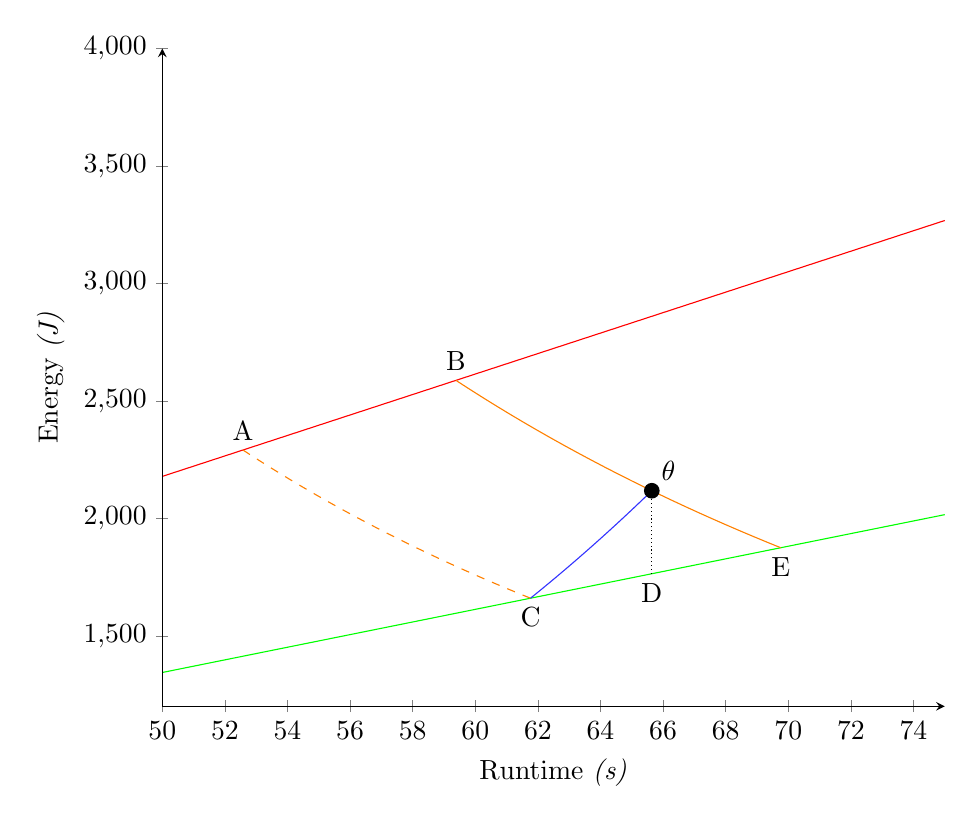
\begin{tikzpicture}
  \providecommand{\plotwidth}{\linewidth}
  \begin{axis}[
    axis on top,
    axis x line=bottom,
    axis y line=left,
  	xlabel={Runtime \emph{(s)}},
    ylabel={Energy \emph{(J)}},    
    xmin=50, xmax=75,
    ymin=1200, ymax=4000,
    width=\plotwidth,
    legend to name=lavamd:legend
    ]

    %% Model Parameters %%
    \pgfmathsetmacro{\baselinepower}{26.876067}
    \pgfmathsetmacro{\rooflinepower}{43.570651}
    \pgfmathsetmacro{\codepower}{32.259372}
    \pgfmathsetmacro{\codetime}{65.640072}
    % Sadly, pgfplots sucks too much to calculate cube roots
    % These values are calculated with a ruby script in tools
    \pgfmathsetmacro{\brnodex}{69.75881800188515}
    \pgfmathsetmacro{\blnodex}{61.764507707810466}
    \pgfmathsetmacro{\trnodex}{59.38220710689976}
    \pgfmathsetmacro{\tlnodex}{52.57704894686994}
    
    %% Intermezzo Values %%
    \pgfmathsetmacro{\brnodey}{\brnodex * \baselinepower}
    \pgfmathsetmacro{\blnodey}{\blnodex * \baselinepower}
    \pgfmathsetmacro{\tlnodey}{\tlnodex * \rooflinepower}
    \pgfmathsetmacro{\trnodey}{\trnodex * \rooflinepower}
    \pgfmathsetmacro{\codeenergy}{\codepower * \codetime}
    \pgfmathsetmacro{\baselineenergy}{\baselinepower * \codetime}

    % arguments: code power, code time, x - todo, apparently not supposed to do pgfmathparse
    \pgfmathdeclarefunction{metricbound}{3}{%
      \pgfmathparse{((#1 * #2^3) / #3^2)}%
    }
    \pgfmathdeclarefunction{definitionbound}{3}{%
      \pgfmathparse{((#1 / #2^3) * #3^4)}%
    }

    % BETA ROOFLINE BOUND 
    \addplot[color=red, domain=\pgfkeysvalueof{/pgfplots/xmin}:\pgfkeysvalueof{/pgfplots/xmax}] {\rooflinepower * x};
    \addlegendentry{$P_{max}$ Energy Bound}

    % ALPHA BASELINE BOUND 
    \addplot[color=green, domain=\pgfkeysvalueof{/pgfplots/xmin}:\pgfkeysvalueof{/pgfplots/xmax}] {\baselinepower * x};
    \addlegendentry{$P_{min}$ Energy Bound} 

    \addplot[color=orange, domain=\trnodex:\brnodex] { metricbound(\codepower, \codetime, x)};
    \addlegendentry{Optimisation Bound}

    \addplot[color=blue!80, domain=\blnodex:\codetime] { definitionbound(\codepower, \codetime, x)};
    \addlegendentry{Contribution Bound}

    \addplot[color=orange, dashed, domain=\tlnodex:\blnodex] {metricbound(\baselinepower, \blnodex, x)};
    \addlegendentry{Optimisation Limit}

    % Constant Time (Vertical) dotted line
    \draw[densely dotted] ({axis cs:\codetime,\baselineenergy}) -- ({axis cs:\codetime,\codeenergy});

    \node[circle,fill,inner sep=2pt] at (axis cs:\codetime,\codeenergy) {};
    \node[above right] at (axis cs:\codetime,\codeenergy) {$\theta$};
    
    \node [above] at ({axis cs:\tlnodex, \tlnodey}) {A};
    \node [above] at ({axis cs:\trnodex, \trnodey}) {B};
    \node [below] at ({axis cs:\blnodex, \blnodey}) {C};
    \node [below] at ({axis cs:\codetime,\baselineenergy}) {D};
    \node [below] at ({axis cs:\brnodex, \brnodey}) {E};
 \end{axis}
\end{tikzpicture}
%
    \caption{LavaMD}%
    \label{fig:lavamd_pose}
  \end{subfigure}%
  \begin{center}%
    \ref{minimd:legend}%
  \end{center}%
  \caption{$E^1t^2$ POSE comparison}%
  \label{fig:comparison}%
\end{figure}


\subsection{POSE Models for Frequency Scaling}
The relationship between P-state and energy consumption is non-linear and workload dependent.
Operating in low power states can increase runtime, offsetting any energy savings from reduced power draw~\cite{le:2010aa}.
Application-aware DVFS can save energy by selecting the optimal P-state schedule for a given code~\cite{choi:2004aa}.
This implies that code changes may effect the optimal P-state assignment. 
We now use POSE to reason about this class of optimisation.

The performance of MiniMD and LavaMD was measured for each P-state supported by our system.
\autoref{fig:pstates} shows that the energy consumption of both codes can be reduced at the cost of increased runtime.
That said, the lowest $E^1t^2$ value for both codes occurs at 3.2 GHz, meaning race-to-halt is the optimal strategy in terms of this metric. 

While useful, this simple analysis fails to account for potential co-opti\-misa\-tion of activity factor and P-state.
It is possible that different optimisations may be required to achieve optimal performance in different P-states.
The flexibility of POSE allows us to model this scenario by considering optimisations which can impact P-state as well as activity factor.
\autoref{eq:pbfreq} gives the feasible performance envelope corresponding to this class of optimisation.

\begin{align}
  \label{eq:pbfreq}
  \begin{split}
    P_{min} &= (1.6\text{ GHz}, \alpha, 4) = 13.51W, \\
    P_{max} &= (3.2\text{ GHz}, \beta, 4) = 49.61W
  \end{split}
\end{align}



\begin{figure}[t]%
\begin{subfigure}[t]{.5\linewidth}%
\centering%
\@ifundefined{pstateminimdtable}{%
  \pgfplotstableread[col sep=comma]{plot/minimd-pstates/data/pstate_power_4_cores.csv}\pstateminimdtable
}{}

\begin{tikzpicture}
  \begin{axis}[
    width=0.75\linewidth,
    axis on top,
    axis x line=bottom,
    axis y line=left,
    xlabel={Runtime (\emph{s})},
    ylabel={Energy (\emph{J})},    
    xmin=20, xmax=65,
    ymin=200, ymax=1200,
    legend columns=2,
    legend to name=minimd-pstate:legend,
    legend style={/tikz/every even column/.append style={column sep=0.2cm}} % space out columns a bit
    ]

    % arguments: code power, code time, x, n 
    \pgfmathdeclarefunction{metricbound}{4}{%
      \pgfmathparse{((#1 * #2^(#4 + 1)) / #3^#4)}%
    }
    \pgfmathdeclarefunction{definitionbound}{4}{%
      \pgfmathparse{((#1 / #2^(#4 + 1)) * #3^(#4 + 2))}%
    }

    %%
    \pgfmathsetmacro{\codetime}{31.160996}
    \pgfmathsetmacro{\codepower}{26.555410070974624}
    \pgfmathsetmacro{\blnodex}{24.876044579784466}
    \addplot[black, densely dotted, domain=\blnodex:\codetime, forget plot] {definitionbound(\codepower, \codetime, x, 2)};

    %%
    \pgfmathsetmacro{\codetime}{32.221644}
    \pgfmathsetmacro{\codepower}{25.19066851461707}
    \pgfmathsetmacro{\blnodex}{26.17914532437151}
    \addplot[black, densely dotted, domain=\blnodex:\codetime, forget plot] {definitionbound(\codepower, \codetime, x, 2)};

    %%
    \pgfmathsetmacro{\codetime}{33.189564}
    \pgfmathsetmacro{\codepower}{24.052689996168674}
    \pgfmathsetmacro{\blnodex}{27.384280155637242}
    \addplot[black, densely dotted, domain=\blnodex:\codetime, forget plot] {definitionbound(\codepower, \codetime, x, 2)};

    %%
    \pgfmathsetmacro{\codetime}{35.548669}
    \pgfmathsetmacro{\codepower}{21.708309894809283}
    \pgfmathsetmacro{\blnodex}{30.35072062021389}
    \addplot[black, densely dotted, domain=\blnodex:\codetime, forget plot] {definitionbound(\codepower, \codetime, x, 2)};

    %%
    \pgfmathsetmacro{\codetime}{36.852917}
    \pgfmathsetmacro{\codepower}{20.791885293639034}
    \pgfmathsetmacro{\blnodex}{31.919904165043228}
    \addplot[black, densely dotted, domain=\blnodex:\codetime, forget plot] {definitionbound(\codepower, \codetime, x, 2)};

    %%
    \pgfmathsetmacro{\codetime}{38.225746}
    \pgfmathsetmacro{\codepower}{19.926273930664426}
    \pgfmathsetmacro{\blnodex}{33.58161699951163}
    \addplot[black, densely dotted, domain=\blnodex:\codetime, forget plot] {definitionbound(\codepower, \codetime, x, 2)};

    %%
    \pgfmathsetmacro{\codetime}{39.720356}
    \pgfmathsetmacro{\codepower}{19.032817706870503}
    \pgfmathsetmacro{\blnodex}{35.432334683311204}
    \addplot[black, densely dotted, domain=\blnodex:\codetime, forget plot] {definitionbound(\codepower, \codetime, x, 2)};

    %%
    \pgfmathsetmacro{\codetime}{41.430395}
    \pgfmathsetmacro{\codepower}{18.26008617586195}
    \pgfmathsetmacro{\blnodex}{37.47190734697387}
    \addplot[black, densely dotted, domain=\blnodex:\codetime, forget plot] {definitionbound(\codepower, \codetime, x, 2)};

    %%
    \pgfmathsetmacro{\codetime}{45.85507}
    \pgfmathsetmacro{\codepower}{16.61222678321067}
    \pgfmathsetmacro{\blnodex}{42.802165661611}
    \addplot[black, densely dotted, domain=\blnodex:\codetime, forget plot] {definitionbound(\codepower, \codetime, x, 2)};

    %%
    \pgfmathsetmacro{\codetime}{49.7305}
    \pgfmathsetmacro{\codepower}{15.67846259337831}
    \pgfmathsetmacro{\blnodex}{47.323406701270244}
    \addplot[black, densely dotted, domain=\blnodex:\codetime, forget plot] {definitionbound(\codepower, \codetime, x, 2)};

    %%
    \pgfmathsetmacro{\codetime}{52.358683}
    \pgfmathsetmacro{\codepower}{15.137478343372388}
    \pgfmathsetmacro{\blnodex}{50.41098720057872}
    \addplot[black, densely dotted, domain=\blnodex:\codetime, forget plot] {definitionbound(\codepower, \codetime, x, 2)};

    %%
    \pgfmathsetmacro{\codetime}{55.340763}
    \pgfmathsetmacro{\codepower}{14.650088958838532}
    \pgfmathsetmacro{\blnodex}{53.866578212248804}
    \addplot[black, densely dotted, domain=\blnodex:\codetime, forget plot] {definitionbound(\codepower, \codetime, x, 2)};

    %%
    \pgfmathsetmacro{\codetime}{58.637567}
    \pgfmathsetmacro{\codepower}{14.09304050763225}
    \pgfmathsetmacro{\blnodex}{57.81786383949271}
    \addplot[black, densely dotted, domain=\blnodex:\codetime, forget plot] {definitionbound(\codepower, \codetime, x, 2)};


    %% Model Parameters %%
    \pgfplotstablegetelem{0}{Runtime}\of{\pstateminimdtable}
    \pgfmathsetmacro{\codetime}{\pgfplotsretval} 
    \pgfplotstablegetelem{0}{Energy}\of{\pstateminimdtable}
    \pgfmathsetmacro{\codeenergy}{\pgfplotsretval} 
    \pgfmathsetmacro{\baselinepower}{13.510238}

    %% Intermezzo Values %%
    \pgfmathsetmacro{\codepower}{\codeenergy / \codetime}



    % ALPHA BASELINE BOUND 
    \addplot[color=printgreen, very thick, name path=basebound, domain=\pgfkeysvalueof{/pgfplots/xmin}:\pgfkeysvalueof{/pgfplots/xmax}] {\baselinepower * x};
    \addlegendentry{$P_{min}$ Energy Bound} 


    %% 3.2 GHz start point
    \pgfmathsetmacro{\blnodex}{23.77199310523716}
    \pgfmathsetmacro{\brnodex}{38.6049404590049}
    \addplot[name path=edpdef, darkgray, thick, domain=\blnodex:\codetime, forget plot] {definitionbound(\codepower, \codetime, x, 2)};
    \addplot[name path=edpopt, darkgray, thick, domain=\codetime:\brnodex] {metricbound(\codepower, \codetime, x, 2)};
    \addlegendentry{3.2 GHz POSE}

    % 2.2 GHz non-overlapping pose
    \pgfmathsetmacro{\codetime}{43.161913}
    \pgfmathsetmacro{\codepower}{17.552650110758528}
    \pgfmathsetmacro{\blnodex}{39.55555231782452}
    \pgfmathsetmacro{\brnodex}{47.097072968441026}
    \addplot[name path=edpdef, gray, thick, domain=\blnodex:\codetime, forget plot] {definitionbound(\codepower, \codetime, x, 2)};
    \addplot[name path=edpopt, gray, thick, domain=\codetime:\brnodex] {metricbound(\codepower, \codetime, x, 2)};
    \addlegendentry{First Non-Overlapping POSE}
    
    %% PState progression
    \tikzset{ every pin edge/.append style={thick} }
    \addplot[mark=x, black, only marks] table[x=Runtime,y=Energy, trim cells=true] {\pstateminimdtable}
      node[pos=0.0, pin=above:3.2 GHz]{}
      node[pos=1.0, pin=above:1.6 GHz]{}
      node[pos=0.64285714285, pin=above:2.2 GHz]{} % pos is elem index / rows - 1 (zero indexed)
      % How to specify pin length (.15cm) and angle (120)
      %node[pos=0.5745, pin={[pin distance=0.15cm] 120:2.2 GHz}]{}
    ;
    \addlegendentry{P-state Measurement}
 \end{axis}
\end{tikzpicture}
%
\caption{MiniMD}%
\label{fig:minimd-pstates}%
\end{subfigure}%
\begin{subfigure}[t]{.5\linewidth}%
\@ifundefined{pstatelavamdtable}{%
  \pgfplotstableread[col sep=comma]{plot/lavamd-pstates/data/pstate_power_4_cores.csv}\pstatelavamdtable
}{}

\begin{tikzpicture}
  \begin{axis}[
    width=0.95\linewidth,
    axis on top,
    axis x line=bottom,
    axis y line=left,
  	xlabel={Runtime \emph{(s)}},
    ylabel={Energy \emph{(J)}},    
    xmin=0, xmax=140,
    ymin=0, ymax=3800,
    legend columns=2,
    legend to name=lavamd-pstate:legend,
    legend style={/tikz/every even column/.append style={column sep=0.2cm}} % space out columns a bit
    ]

    %% Model Parameters %%
    \pgfplotstablegetelem{0}{Runtime}\of{\pstatelavamdtable}
    \pgfmathsetmacro{\codetime}{\pgfplotsretval} 
    \pgfplotstablegetelem{0}{Energy}\of{\pstatelavamdtable}
    \pgfmathsetmacro{\codeenergy}{\pgfplotsretval} 
    \pgfmathsetmacro{\baselinepower}{13.510238}

    %% Intermezzo Values %%
    \pgfmathsetmacro{\codepower}{\codeenergy / \codetime}

    % arguments: code power, code time, x, n 
    \pgfmathdeclarefunction{metricbound}{4}{%
      \pgfmathparse{((#1 * #2^(#4 + 1)) / #3^#4)}%
    }
    \pgfmathdeclarefunction{definitionbound}{4}{%
      \pgfmathparse{((#1 / #2^(#4 + 1)) * #3^(#4 + 2))}%
    }

    % ALPHA BASELINE BOUND 
    \addplot[color=green, name path=basebound, domain=\pgfkeysvalueof{/pgfplots/xmin}:\pgfkeysvalueof{/pgfplots/xmax}] {\baselinepower * x};
    \addlegendentry{$P_{min}$ Energy Bound} 


    %% 3.2 GHz start point
    \pgfmathsetmacro{\brnodex}{87.73374843784023}
    \pgfmathsetmacro{\blnodex}{49.11016716922632}
    \addplot[name path=edpdef, draw=none, domain=\blnodex:\codetime+1, forget plot] {definitionbound(\codepower, \codetime, x, 2)};
    \addplot[name path=edpopt, draw=none, domain=\codetime-1:\brnodex, forget plot] {metricbound(\codepower, \codetime, x, 2)};

    \path[name path=edpspace,
      intersection segments={
        of=edpdef and edpopt,
        sequence=A0 -- B1,
      }
      ]; 
    \addplot[blue!20] fill between[of=edpspace and basebound]; 
    \addlegendentry{3.2 GHz POSE}

    %% PState progression
    \addplot[mark=x, black] table[x=Runtime,y=Energy, trim cells=true] {\pstatelavamdtable}
      node[pos=0.0, pin=left:3.2 GHz]{}
      node[pos=1.0, pin=95:1.6 GHz]{}
      node[pos=0.636, pin={[pin distance=0.15cm] above:2.1 GHz}]{}
    ;
    \addlegendentry{P-State Progression}


    %%
    \pgfmathsetmacro{\codetime}{67.788671}
    \pgfmathsetmacro{\codepower}{30.534496154969613}
    \pgfmathsetmacro{\blnodex}{51.65525781584337}
    \addplot[name path=edpdef, gray, densely dashed, domain=\blnodex:\codetime, forget plot] {definitionbound(\codepower, \codetime, x, 2)};

    %%
    \pgfmathsetmacro{\codetime}{69.909725}
    \pgfmathsetmacro{\codepower}{28.972621505806238}
    \pgfmathsetmacro{\blnodex}{54.21207070239038}
    \addplot[name path=edpdef, gray, densely dashed, domain=\blnodex:\codetime, forget plot] {definitionbound(\codepower, \codetime, x, 2)};

    %%
    \pgfmathsetmacro{\codetime}{72.820343}
    \pgfmathsetmacro{\codepower}{27.23156518227331}
    \pgfmathsetmacro{\blnodex}{57.647815146592066}
    \addplot[name path=edpdef, gray, densely dashed, domain=\blnodex:\codetime, forget plot] {definitionbound(\codepower, \codetime, x, 2)};

    %%
    \pgfmathsetmacro{\codetime}{78.83738}
    \pgfmathsetmacro{\codepower}{24.363863791516156}
    \pgfmathsetmacro{\blnodex}{64.76958711476986}
    \addplot[name path=edpdef, gray, densely dashed, domain=\blnodex:\codetime, forget plot] {definitionbound(\codepower, \codetime, x, 2)};

    %%
    \pgfmathsetmacro{\codetime}{80.443575}
    \pgfmathsetmacro{\codepower}{23.569310575766927}
    \pgfmathsetmacro{\blnodex}{66.82363092159444}
    \addplot[name path=edpdef, gray, densely dashed, domain=\blnodex:\codetime, forget plot] {definitionbound(\codepower, \codetime, x, 2)};

    %%
    \pgfmathsetmacro{\codetime}{83.583275}
    \pgfmathsetmacro{\codepower}{22.42571518045925}
    \pgfmathsetmacro{\blnodex}{70.59245458487962}
    \addplot[name path=edpdef, gray, densely dashed, domain=\blnodex:\codetime, forget plot] {definitionbound(\codepower, \codetime, x, 2)};

    %%
    \pgfmathsetmacro{\codetime}{87.25231}
    \pgfmathsetmacro{\codepower}{21.415643975500476}
    \pgfmathsetmacro{\blnodex}{74.83203474018039}
    \addplot[name path=edpdef, gray, densely dashed, domain=\blnodex:\codetime, forget plot] {definitionbound(\codepower, \codetime, x, 2)};

    %%
    \pgfmathsetmacro{\codetime}{90.581583}
    \pgfmathsetmacro{\codepower}{20.54295973167084}
    \pgfmathsetmacro{\blnodex}{78.77224707386881}
    \addplot[name path=edpdef, gray, densely dashed, domain=\blnodex:\codetime, forget plot] {definitionbound(\codepower, \codetime, x, 2)};

    %%
    \pgfmathsetmacro{\codetime}{95.357508}
    \pgfmathsetmacro{\codepower}{19.637888418812288}
    \pgfmathsetmacro{\blnodex}{84.1803958382032}
    \addplot[name path=edpdef, gray, densely dashed, domain=\blnodex:\codetime, forget plot] {definitionbound(\codepower, \codetime, x, 2)};

    %%
    \pgfmathsetmacro{\codetime}{99.502899}
    \pgfmathsetmacro{\codepower}{18.820670933416725}
    \pgfmathsetmacro{\blnodex}{89.0932975465577}
    \addplot[name path=edpdef, red, densely dashed, domain=\blnodex:\codetime] {definitionbound(\codepower, \codetime, x, 2)};
    \addlegendentry{Optimisation Cutoff}
    %%
    \pgfmathsetmacro{\codetime}{109.970804}
    \pgfmathsetmacro{\codepower}{17.334285425429826}
    \pgfmathsetmacro{\blnodex}{101.20370662532102}
    \addplot[name path=edpdef, gray, densely dashed, domain=\blnodex:\codetime, forget plot] {definitionbound(\codepower, \codetime, x, 2)};

    %%
    \pgfmathsetmacro{\codetime}{115.469869}
    \pgfmathsetmacro{\codepower}{16.703561489274747}
    \pgfmathsetmacro{\blnodex}{107.58539357794623}
    \addplot[name path=edpdef, gray, densely dashed, domain=\blnodex:\codetime, forget plot] {definitionbound(\codepower, \codetime, x, 2)};

    %%
    \pgfmathsetmacro{\codetime}{123.182269}
    \pgfmathsetmacro{\codepower}{16.060352379123653}
    \pgfmathsetmacro{\blnodex}{116.28334319474206}
    \addplot[name path=edpdef, gray, densely dashed, domain=\blnodex:\codetime, forget plot] {definitionbound(\codepower, \codetime, x, 2)};

    %%
    \pgfmathsetmacro{\codetime}{130.924339}
    \pgfmathsetmacro{\codepower}{15.486518591474423}
    \pgfmathsetmacro{\blnodex}{125.09985043035239}
    \addplot[name path=edpdef, gray, densely dashed, domain=\blnodex:\codetime, forget plot] {definitionbound(\codepower, \codetime, x, 2)};
  \end{axis}
\end{tikzpicture}
%
\caption{LavaMD}%
\label{fig:lavamd-pstates}%
\end{subfigure}%
\begin{center}%
\ref{minimd-pstate:legend}%
\end{center}%
\caption{$E^1t^2$ POSE for P-state Optimisation}%
\label{fig:pstates}%
\end{figure}%

We choose the 3.2 GHz run as our initial `unoptimised' baseline because this is the P-state our system defaults to when running MiniMD or LavaMD.
If the POSE models for two P-states do not overlap then switching to the higher performance P-state beats any possible power optimisation at the weaker state.
This state can then be excluded from any search for power optimisations.

For MiniMD, \autoref{fig:minimd-pstates} shows that the first POSE model which does not overlap with the one built for our baseline occurs at 2.2 GHz.
This means no power optimisations exists at P-states 2.2 GHz and below which can match the $E^1t^2$ performance of our unoptimised baseline.
Conversely, such an optimisation may exist at frequencies between 3.2 GHz and 2.2 GHz as shown by the overlapping of the respective POSE models.
For LavaMD this optimisation threshold is slightly lower at 2.1 GHz, lending support to the claim that of these two codes LavaMD is more amenable to power optimisation.

Dynamic Concurrency Throttling has also been proposed as a means to reduce energy consumption~\cite{maury:2006aa}.
It would be trivial to use POSE to model optimisations which influence core count.
The only difference between this and our DVFS investigation would be slightly different parameterisation of the feasible performance envelope ($C_{min}=1$).
